\chapter {Marco Teórico}

\section {Extracción y descripción de características}

Las características de los objetos son cualidades que nos servirán para identificarlos dentro de una imagen donde pueden existir objetos similares. Para poder discernir de los objetos que estén en la imagen nos basamos en las características encontradas, que serán encapsuladas en un descriptor. Un descriptor de un objeto es la representación, de una manera reducida, de todas las características que se pueden obtener de toda la información del objeto, esto facilitara la comparación entre los diferentes objetos que existan en una imagen.

Para extraer las características existen diferentes formas, dependerá de que algoritmo se utilice, cada uno de ellos se enfoca en encontrar características como esquinas, bordes ,crestas y regiones que son más obscuras o más claras; no todos los reconocedores encontraran las mismas o todos los tipos de características. Para que estos puntos sean robustos deben poder ser encontrados aun que los objetos se encuentren rotados, escalados, con camios de iluminación o hasta estén parcialmente ocluidos.

En el capitulo 3, se explicara como se obtienen los puntos característicos por medio del algoritmo de SIFT (Scale-Invariant Feature Transform).


\pagebreak

\section {Computo en GPU's}

Hasta hace 12 años la velocidad a la que crecían cada generación de procesadores era increíble, los programas eran tan rápidos como cada nueva generación de procesadores. Este crecimiento entre cada generación se detuvo, el problema es el consumo de energía y la disipación de calor, no permiten aumentar la frecuencia del reloj del procesador y el nivel de actividades por ciclo, en una sola unidad de procesamiento (CPU). Todos los productores de procesadores migraron a un nuevo modelo, los procesadores multinúcleo incrementaron el poder de procesamiento.

\begin{figure}[ph]
			\centering
				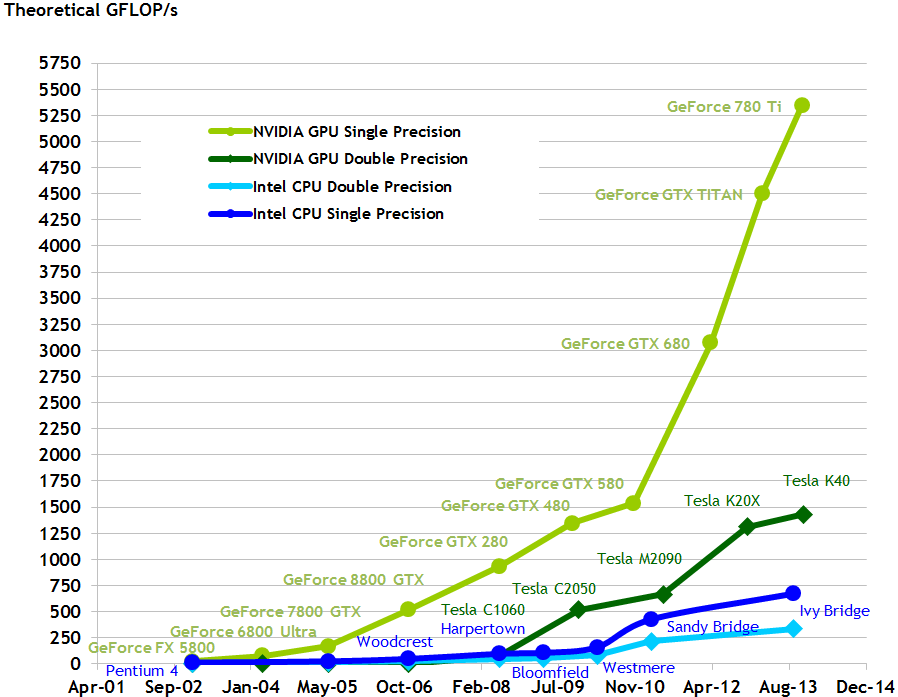
\includegraphics[scale=0.7]{img/flops.png}
			\caption{Comparación entre GPU vs CPU \cite{Flops} }
\end{figure}

Este cambio en los procesadores tuvo un gran impacto a los programadores, la mayoría de las aplicaciones son escritas de forma secuencial,  por que la ejecución de estas son comprensibles paso a paso, mediante el código. Pero un programa secuencial ejecutándose en un solo núcleo del procesador, no sera más rápido. Entonces los programadores ya no pueden agregar cualidades y capacidades a sus programas.


Llega el momento de cambiar, si se desea que la calidad de los programas siga escalando con cada generación de procesadores, se deben crear programas que trabajen con múltiples hilos, cooperando todos para completar un trabajo más rápido. 

Existen dos corrientes principales en cuanto a los procesadores multinúcleo, el primero, es donde se pretende mantener la velocidad de los programas secuenciales, mientras se mueven entre múltiples núcleos; la segunda, se centra más en la ejecución de aplicaciones en paralelo, tiene un gran numero de núcleos pequeños que va creciendo con cada generación. Es esta rama en la que entran las unidades de procesamiento gráfico o por sus siglas en ingles GPU.\cite{Kirk2010} 

En el capitulo 4 hablaremos más a detalle sobre el computo en GPU especialmente de los GP-GPU de Nvidia.


